%
% File naaclhlt2010.tex
%
% Contact: nasmith@cs.cmu.edu

\documentclass[11pt,letterpaper]{article}
\usepackage{naaclhlt2010}
\usepackage{times}
\usepackage{latexsym}
\setlength\titlebox{4cm}    % Expanding the titlebox
\usepackage{tikz}
\usepackage{amsmath}
\usepackage{algorithm}% http://ctan.org/pkg/algorithm
\usepackage{algpseudocode}
\usepackage{caption}
\usepackage{subfigure}
\usepackage{enumerate}
\usepackage{url}

\graphicspath{ {images/} }

\DeclareMathOperator*{\argmax}{\arg\!\max}

\title{\huge Phase-Based RNN Decoder}

\author{Haitang Hu, \ Yating Jing\\
  \tt hthu,\,yating@jhu.edu}
\date{}

\begin{document}
\maketitle

\begin{abstract}
In this project, a RNN Encoder-Decoder is used to rescore the translation model scores based on existing phrase table. The RNN Encoder-Decoder consists of two recursive networks which can encodes the input sequences based on history and a bilingual word embedding, and decodes corresponding representations into output sequences respectively. The two networks are jointly trained using negative log-likelihood as the objective function, with sentence level mini-batch SGD. Due to the substantial amount of time required to train the model, we only conducted experiments on small data set.
\end{abstract}

\section{Introduction}
In the realm of machine translation, decoding is one of the most important tasks. A decoder takes a source sentence as input, then finds its best target translation under the decoding model. The decoder is trained to maximize the conditional probability of a target (English) sentence $\mathbf{e}$ given a source (Foreign) sentence $\mathbf{f}$. 
\begin{equation}
\begin{split}
\mathbf{e^*} &= \arg \ \underset{\mathbf{e}}{\max}\text{ } p(\mathbf{e}\mid \mathbf{f}) \\
&=  p_{TM}(\mathbf{e}\mid \mathbf{f}) \times p_{LM}(\mathbf{e})
\end{split}
\end{equation}
where \textit{TM} represents a phrased-based translation model and \textit{LM} denotes an n-gram language model, as described in \cite{phi}. 

Deep neural networks are becoming increasingly popular in the area of natural language processing and have shown significant success. The RNN encoder-decoder model proposed in \cite{rnn} maps a variable-length source sentence to a fixed-length vector and then decodes and maps the vector back to a variable-length target sentence. By jointly training two recursive neural networks, the conditional probability of the target sentence given the source sentence is then maximized. The empirical evaluation conducted in \cite{rnn} shows significant performance improvement. 

The primary goal is to integrate the Recursive Neural Network into the phrase-based translation model, use a RNN Encoder-Decoder to evaluate the translation probability $p_{TM}(\mathbf{e}\mid \mathbf{f})$. 

\section{Recurrent Neural Network}
\subsection{Introduction to RNN}
A recurrent neural network(RNN) consists of an input layer $\mathbf{x}$, hidden layer $\mathbf{h}$ and an output layer $\mathbf{y}$, which operates on a variable-length sequence $\mathbf{x} = (x_1, \dots, x_t)$, where $x_t$ denotes the input variable at time step $t$. At each time $t$, the hidden layer $\mathbf{h}^{(t)} $ is updated by 
\begin{equation}
\mathbf{h}^{(t)} = f(\mathbf{h}^{(t-1)}, x_t)
\end{equation}
where $f$ could be non-linear activation function or a long short-term memory(LSTM).

Considering the behavior of the RNN, at time $t$, the hidden state $h_t$ encodes all the history from $1 \to t-1$.

Given an observed sequence $X$(a sequence of words), each word fully depends on all the preceding words, because the current hidden status $h_t$ could capture all history preceding current time step. So the probability of observing sequence $\mathbf{x}$ can be written as
\begin{equation}
p(\mathbf{x}) = \prod_{t=1}^Tp(x_t \mid x_{t-1},\dots, x_1)
\end{equation}
For a specific $x_t$, the probability of emitting the $j$th word in Vocabulary $K$ is  then
$$ p(x_t, e_t=j \mid x_{t-1}, \dots, 1)$$ 

The distribution over $\mathbf{x}$ then becomes a multinomial distribution over $K$ possible outputs, thereby the \textit{softmax} would be an intuitive choice. Additionaly, since $x_t$ could get all historical dependencies on hidden state $h_t$, each output word is represented as a word vector using $1$-of-$K$ encoding:
\begin{equation}
p(x_{t,j} = 1 \mid x_{t-1}, \dots, x_1) = \frac{\exp\{w_j h_t\}}{\sum\limits_{k=1}^K \exp\{w_k h_t\}}
\end{equation}
where $K$ is the size of the vocabulary.

\subsection{Auto Encoder-Decoder}

The basic structure of the RNN Encoder-Decoder is illustrated in Figure 1. Note that in length of the input vector $T$ is not necessarily equal to the length of the output vector $T^\prime$. 

\begin{figure}[H]
	\begin{center}
\usetikzlibrary{arrows}
\usetikzlibrary{shapes}
\begin{tikzpicture} 
\begin{scope}
	\tikzstyle{every node}=[minimum size=0.6pt, align=center]
	\node (x1) at (-1.4,0) {$\mathbf{x}_1$};
	\node (x2) at (-1.4,-1.4) {$\mathbf{x}_2$};
	\node (xt) at (-1.4, -4.2) {$\mathbf{x}_T$};
	\node[draw, circle] (h1) at (0, 0) {$\mathbf{h}_1$};
	\node[draw, circle] (h2) at (0,-1.4) {$\mathbf{h}_2$};
	\node (sus) at (0, -2.8) {$\mathbf{\vdots}$};
	\node[draw, circle] (ht) at (0, -4.2) {$\mathbf{h}_T$};
			
	\node[draw, circle] (c) at (1, -5.6) {$\mathbf{c}$};
	
	\node[draw, circle] (oh1) at (2.4, -4.2) {$\mathbf{h}_1$};
	\node[draw, circle] (oh2) at (2.4,-2.8) {$\mathbf{h}_2$};
	\node (osus) at (2.4, -1.4) {$\mathbf{\vdots}$};
	\node[draw, circle] (oht) at (2.4, 0) {$\mathbf{h}_{T^\prime}$};
	\node (y1) at (3.8, -4.2) {$\mathbf{y}_1$};
	\node (y2) at (3.8,-2.8) {$\mathbf{y}_2$};
	\node (yt) at (3.8, 0) {$\mathbf{y}_{T^\prime}$};
	
	\draw [line width=1.0pt][-stealth] (x1) -- (h1);
	\draw [line width=1.0pt][-stealth] (h1) -- (h2);
	\draw [line width=1.0pt][-stealth] (x2) -- (h2);
	\draw [line width=1.0pt][-stealth] (h2) -- (sus);
	\draw [line width=1.0pt][-stealth] (sus) -- (ht);
	\draw [line width=1.0pt][-stealth] (xt) -- (ht);
	\draw [line width=1.0pt][-stealth] (ht) -- (c);
	
	\draw [line width=1.0pt][-stealth] (oh1) -- (y1);
	\draw [line width=1.0pt][-stealth] (oh1) -- (oh2);
	\draw [line width=1.0pt][-stealth] (oh2) -- (y2);
	\draw [line width=1.0pt][-stealth] (oh2) -- (osus);
	\draw [line width=1.0pt][-stealth] (osus) -- (oht);
	\draw [line width=1.0pt][-stealth] (oht) -- (yt);
	\draw [line width=1.0pt][-stealth] (y1) -- (y2);
	
	\draw [->, dashed, line width=1.0pt] (c) -- (oh1);
	\draw [->, dashed, line width=1.0pt] (c) -- (oh2);
	\draw [->, dashed, line width=1.0pt] (c) -- (oht);
	\draw [->, dashed] (c) -- (y1);
	\draw [->, dashed] (c) -- (y2);
	\draw [->, dashed] (c) -- (yt);
\end{scope}
\end{tikzpicture}
	\end{center}
	\caption{RNN Encoder-Decoder illustration}
\end{figure}

The \textbf{encoder} is a RNN takes in a variable length input sequence $\mathbf{x}$, and outputs a summary $\mathbf{c}$. More specifically, given an input sequence $\mathbf{x} = (x_1,\dotsc, x_T)$, the update function for the hidden layer $\mathbf{h}^{(t)}$ at time step $t$ is updated using equation (2), where $f$ is the \textit{sigmoid} activation function. 

Afterwards, the hidden states of the RNN are summarized by a summary vector $\mathbf{c}$ of the whole input sequence, that is, the whole history of the sentence is memorized. The summary at the $N^{th}$ step is calculated as below:
\begin{equation}
\mathbf{c} = \tanh(\mathbf{V}\mathbf{h}^{(N)})
\end{equation}
where $\mathbf{V}$ denotes the corresponding weight matrix in the encoder. Note that the summary vector $\mathbf{c}$ is produced when $t = |\mathbf{x}|$.

The \textbf{decoder} takes the trained history summary $\mathbf{c}$ produced by the encoder as the input, generates output sequence $\mathbf{y}$ from its own hidden states $\mathbf{h}^{(t-1)}$. 

More specifically, the decoder RNN predicts the next word $y_t$ given the hidden state $\mathbf{h}^{(t)}$, the preceding word $y_{t-1}$ and the summary $\mathbf{c}$. The update function for the decoder hidden layer at time step $t$ is:
\begin{equation}
\mathbf{h}^{(t)} = f(\mathbf{h}^{(t-1)}, y_{t-1}, \mathbf{c})
\end{equation}

and the conditional probability of the next output word is:
\begin{equation}
p(y_t\mid y_{t-1}, y_{t-2}, \dotsc, y_1, \mathbf{c}) = g (\mathbf{h}^{(t)}, y_{t-1}, \mathbf{c})
\end{equation}
where g is the \textit{softmax} activation function.

The score used to choose the candidate translation is then the log-probability of $\mathbf{y}$:
\begin{equation}
\log p(\mathbf{y}) = \sum\limits_{t=1}^T \, \log p(y_t\mid y_{t-1}, \dotsc , y_1)
\end{equation}

\subsection{Training}
\subsubsection{Back Propagation}
Neural networks can be trained by stochastic gradient descent using back-propagation(BP) algorithm as proposed in \cite{bp}. Assume the weights for input, hidden and output layers are represented by matrices $\mathbf{U}$, $\mathbf{W}$ and $\mathbf{V}$. The weight matrices are adjusted after seeing every example. A cross entropy criterion is used to  obtain gradient of an error vector in the output layer, which is then back-propagated to the hidden layer, then to the input layer. The illustration of one epoch of a simple RNN is shown in Figure 2. 

\begin{figure}[H]
	\begin{center}
\begin{tikzpicture}
\usetikzlibrary{arrows}
\usetikzlibrary{shapes}
\begin{scope}
	\tikzstyle{every node}=[minimum size=0.6pt, align=center]
	\node[draw] (x) at (0,0) {$\mathbf{x}^{(t)}$};
	\node[draw] (h0) at (0,-1.5) {$\mathbf{h}^{(t-1)}$};
	\node[draw] (h) at (2, 0) {$\mathbf{h}^{(t)}$};
	\node[draw] (y) at (4, 0) {$\mathbf{y}^{(t)}$};
	
	\draw [line width=1.0pt][-stealth] (x) -- node[above]{U} ++ (h);
	\draw [line width=1.0pt][-stealth] (h0) -- node[above]{W} ++ (h);
	\draw [line width=1.0pt][-stealth] (h) -- node[above]{V} ++ (y);
	\end{scope}
\end{tikzpicture}
	\end{center}
	\caption{Illustration of one epoch of RNN}
\end{figure}

Since the optimization goal is to maximize the total log-likelihood of the target translation, which is equivalent to minimize the negative log-likelihood. Here define the loss(error term) as the total negative log-likelihood of the current output sequence:
\begin{equation}
\textit{NLL}^{(t)} = -\sum\limits_{i=1}^t \, \log p(y_i\mid y_{i-1}, \dotsc , y_1)
\end{equation}

The gradient of error vector in the output layer $\mathbf{e}_o^{(t)} $ w.r.t a given weight matrix $\mathbf{m}$ at each time step is then:
\begin{equation}
\mathbf{e}_o^{(t)}  = \frac{d}{d \mathbf{m}} \textit{NLL}^{(t)}
\end{equation}
where $\mathbf{m}$ denotes one of the weight matrices $\mathbf{U}$, $\mathbf{W}$, $\mathbf{V}$.

Therefore each element of the weight matrix $\mathbf{V}$ is adjusted as follows:
\begin{equation}
v_{jk}^{(t)} = v_{jk}^{(t-1)}  + \eta\, h_j ^{(t)} e_{ok}^{(t)}
\end{equation}
where $\eta$ is the learning rate and $e_{ok}^{(t)}$ is the error gradient of the $k^{th}$ neuron in the output layer.

Then back propagate the error vector from the output layer to the hidden layer using the equation below:
\begin{equation}
\mathbf{e}_{hj}^{(t)} = {\mathbf{e}_o^{(t)}}^T \mathbf{V}\, h_j^{(t)} (1- h_j^{(t)})
\end{equation}

Next update the weight matrix for the input layer $\mathbf{U}$:
\begin{equation}
u_{ij}^{(t+1)} = u_{ij}^{(t)} + \eta \, x_i^{(t)} e_{hj}^{(t)}
\end{equation}

The update function for the recurrent weight matrix $\mathbf{W}$ is:
\begin{equation}
w_{lj}^{(t+1)} = w_{lj}^{(t)} + \eta \, h_l^{(t-1)} e_{hj}^{(t)}
\end{equation}

\subsubsection{Back Propagation Through time}
For recurrent neural network training, the BP algorithm is not optimal, in that the network only tries to optimiaze the prediction of the next word given the previous word and previous state of the hidden layer. To extend such effect into the future, the short term information stored in the hidden layer can be replaced by some long context information.

According to \cite{bp}, the back-propagation through time(BPTT) training algorithm can ensure that the network will learn what information to be stored in the hidden layer. A RNN with one hidden layer which is used for $N$ time steps can be seen as a deep feedforward network with $N$ hidden layers, which is illustrated in Figure 3, where the unfolding is applied for three time steps.

\begin{figure}[H]
	\begin{center}
\begin{tikzpicture}
\usetikzlibrary{arrows}
\usetikzlibrary{shapes}
\begin{scope}
	\tikzstyle{every node}=[minimum size=0.6pt, align=center]
	\node[draw] (x0) at (-3.6,-3) {$\mathbf{x}^{(t-2)}$};
	\node[draw] (h0) at (-3.6,-4.5) {$\mathbf{h}^{(t-3)}$};
	\node[draw] (x1) at (-1.8,-1.5) {$\mathbf{x}^{(t-1)}$};
	\node[draw] (h1) at (-1.8,-3) {$\mathbf{h}^{(t-2)}$};
	\node[draw] (x2) at (0,0) {$\mathbf{x}^{(t)}$};
	\node[draw] (h2) at (0,-1.5) {$\mathbf{h}^{(t-1)}$};
	\node[draw] (h) at (1.8, 0) {$\mathbf{h}^{(t)}$};
	\node[draw] (y) at (3.2, 0) {$\mathbf{y}^{(t)}$};
	
	\draw [line width=1.0pt][-stealth] (h0) -- node[above]{W} ++ (h1);
	\draw [line width=1.0pt][-stealth] (x0) -- node[above]{U} ++ (h1);
	\draw [line width=1.0pt][-stealth] (h1) -- node[above]{W} ++ (h2);
	\draw [line width=1.0pt][-stealth] (x1) -- node[above]{U} ++ (h2);
	\draw [line width=1.0pt][-stealth] (x2) -- node[above]{U} ++ (h);
	\draw [line width=1.0pt][-stealth] (h2) -- node[above]{W} ++ (h);
	\draw [line width=1.0pt][-stealth] (h) -- node[above]{V} ++ (y);
	\end{scope}
\end{tikzpicture}
	\end{center}
	\caption{Illustration of one epoch of RNN as a deep feedforward network}
\end{figure}

In such RNN errors are propagated from the hidden layer $\mathbf{h}^{(t)}$ to the hidden layer from the previous time step recurrently as follows:
\begin{equation}
\mathbf{e}_h^{(t-\tau-1)} = d_h ({\mathbf{e}_h^{(t-\tau)}}^{T} \mathbf{W}, t-\tau-1)
\end{equation}
where the error vector is obtained using element-wise function $d_h()$:
\begin{equation}
d_{hj}(x, t) = x h_j^{(t)} (1- h_j^{(t)})
\end{equation}
This unfolding process can be applied for as many time steps as many training samples were already seen, however a certain number of steps of unfolding would be sufficient since error gradients quickly vanish as back-propagated in time.

The weight matrix $\mathbf{U}$ between the input layer and hidden layer is then updated as:
\begin{equation}
u_{ij}^{(t+1)} = u_{ij}^{(t)} + \sum\limits_{\tau=0}^T \eta \, x_i^{(t-\tau)} e_{hj}^{(t-\tau)}
\end{equation}
where $\eta$ is the learning rate. Note that $\mathbf{U}$ must be updated in one large change instead of during an incremental changing process, which can lead to instability. 

The update function for the recurrent weight matrix $\mathbf{W}$ is then:
\begin{equation}
w_{lj}^{(t+1)} = w_{lj}^{(t)} + \sum\limits_{\tau=0}^T  \eta \, h_l^{(t-\tau-1)} e_{hj}^{(t-\tau)}
\end{equation}

\subsubsection{Long-Short Term Memory}
In addition to the model architecture described above, a simplified version of long-short term memory(LSTM) units are adopted as the hidden units of the RNN, according to \cite{rnn}, as depicted in Figure 4.
\begin{figure}[ht]
  \centering
    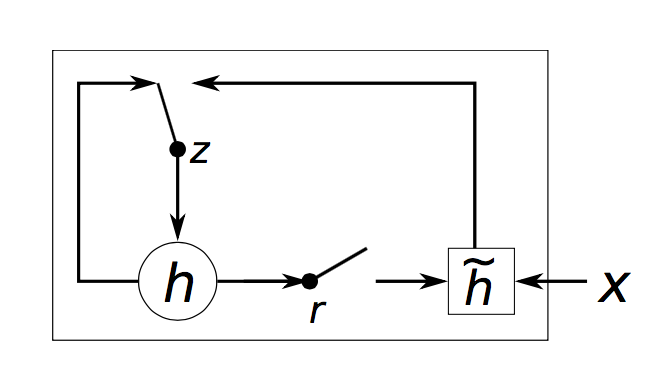
\includegraphics[width=0.45\textwidth]{lstm.png}
    \caption{Illustration of hidden activation function}
\end{figure}

Namely, the reset gate allows the hidden units to drop any irrelevant information by reseting and the update gate decides how much information from previous hidden states should be passed on. When the reset gate is close to 0, the hidden state would ignore the hidden states from previous time steps, reset with current input, and learn to capture the short-term dependencies. On the other hand, those with frequently activated update gates tend to capture long-term dependencies.

More specifically, for the encoder, the activation of the $j^{th}$ hidden unit is computed using a \textit{reset} gate $r_j$ and an \textit{update} gate $z_j$. The two gates are computed as below:

\begin{equation}
\begin{split}
r_j &= \sigma \left({[\mathbf{W}_r\, e(x_t)]}_j + {[\mathbf{U}_r \mathbf{h}^{(t-1)}]}_j \right) \\
z_j &= \sigma \left({[\mathbf{W}_z\, e(x_t)]}_j + {[\mathbf{U}_z \mathbf{h}^{(t-1)}]}_j \right)
\end{split}
\end{equation}

where $\sigma$ is the logistic sigmoid function and $e(x_t)$ denotes the embedding of each input word $x_t$. Weight matrices $\mathbf{W}_r, \mathbf{U}_r, \mathbf{W}_z, \mathbf{U}_z$ are learned during training.

The actual activation of a unit $h_j$ of the encoder is then computed as follows:
\begin{equation}
h_j^{(t)} = z_j h_j^{(t-1)} + (1-z_j)\, \tilde{h}_j^{(t)}  
\end{equation}
where 
\begin{equation}
\tilde{h}_j^{(t)} = \tanh \left( {[\mathbf{W} e(x_t)]}_j +{[\mathbf{U} (\mathbf{r} \odot \mathbf{h}^{(t-1)})]}_j \right)
\end{equation}
where $\odot$ denotes element-wise multiplication. In particular, the initial hidden state $h_j^{(t)}$ is fixed to 0.

For decoder, the \textit{reset} gate $r_j^\prime$ and an \textit{update} gate $z_j^\prime$ are computed as:

\begin{equation}
\begin{split}
r_j^\prime &= \sigma \left({[\mathbf{W}_r^\prime e(y_{t-1})]}_j + {[\mathbf{U}_r^\prime {\mathbf{h}^\prime}^{(t-1)}]}_j + {[\mathbf{C}_r \mathbf{c}]}_j \right) \\
z_j^\prime &= \sigma \left({[\mathbf{W}_z^\prime e(y_{t-1})]}_j + {[\mathbf{U}_z^\prime {\mathbf{h}^\prime}^{(t-1)}]}_j + {[\mathbf{C}_z \mathbf{c}]}_j \right)
\end{split}
\end{equation}
where $e(y_{t})$ denotes the embedding of each output word $y_t$. Weight matrices $\mathbf{W}_r^\prime$, $\mathbf{U}_r^\prime$, $\mathbf{W}_z^\prime$, $\mathbf{U}_z^\prime$, $\mathbf{C}_r$, $\mathbf{C}_z$ are learned during training.

The actual activation of a unit $h_j$ of the decoder is then:
\begin{equation}
{h^\prime}_j^{(t)} = z_j^\prime {h_j^\prime}^{(t-1)} + (1-z^\prime_j)\, \tilde{h}_j^{(t)}  
\end{equation}
where 
\begin{equation}
\tilde{h}_j^{(t)} = \tanh \left( {[\mathbf{W}^\prime e(y_{t-1})]}_j + r_j^\prime  {[\mathbf{U}^\prime {\mathbf{h}^\prime}^{(t-1)} \mathbf{C} \mathbf{c}]} \right)
\end{equation}

According to \cite{rnn}, such hidden units are crucial in getting meaningful result.

\section{Overall model structure}
\subsection{Word Embedding}
We adopted word embeddings to project to and map back from a sequence of words into a continuous space vector: $W: words \rightarrow \mathcal{R}^n$. In other words, a sequence of words is mapped into some high-dimensional vector parameterized by a matrix $\theta$, which each row representing a word:
\begin{equation}
W_\theta(w_n) = \theta_n
\end{equation}
where $W$ is initialized to have one-hot vectors for each word. It then learns to have the meaningful vectors during training. 

In our model, we used a 500-dimension vector for each word. The input matrix fed into the hidden layer is thus the word embedding matrix learned by the RNN encoder-decoder.

\subsection{Max-Pooling}
We applied \textit{Max-Pooling} between our \textit{hidden layer} and \textit{output layer}. Each two adjacent output from hidden layer will be combined to be a new output, where the maximum of those two will be chosen.
\begin{equation}
s_i = \max \{s_{2i-1}, s_{2i} \}
\end{equation}

\subsection{Layers Definition}
The layers of the RNN encoder-decoder are illustrated in Figure 5. At each time step, the source word would be passed through the input layer of the encoder, then the hidden layer of the encoder. In particular, the encoder needs to memorize previous states of its hidden layer $\mathbf{h}^{(t-1)}$ when calculating the current hidden units. 

At time step $t = |\mathbf{x}|$, the information of the entire input sentence is then passed as a summary vector from the encoder to the hidden layer ${\mathbf{h}^\prime}^{(t)}$ of the decoder, then to the max-pooling layer and finally to the output layer.
The functions of each layer are listed below:
\begin{enumerate}[a.]
\item Encoder input layer: word embedding
\item Encoder hidden layer: sigmoid function
\item Decoder hidden layer: sigmoid function
\item Decoder max-out unit: max-pooling
\item Decoder output layer: softmax function
\end{enumerate}

\begin{figure}[H]
	\begin{center}
\begin{tikzpicture}
\usetikzlibrary{arrows}
\usetikzlibrary{shapes}
\begin{scope}
	\tikzstyle{every node}=[minimum size=0.6pt, align=center]
	\node[draw, label=above:$input$] (x) at (-0.8,0) {$\mathbf{x}^{(t)}$};
	\node[draw, label=below:$history$] (h0) at (-0.8,-1.5) {$\mathbf{h}^{(t-1)}$};
	\node[draw, label=above:$hidden $] (h) at (1, 0) {$\mathbf{h}^{(t)}$};
	\node[draw, label=above:$hidden $] (s) at (3, 0) {${\mathbf{h}^\prime}^{(t)}$};
	\node[draw, label=below:$max-pooling$] (o) at (3, -1.5) {${\mathbf{m}}^{(t)}$};
	\node[draw, label=above:$output $] (y) at (5, 0) {$\mathbf{y}^{(t)}$};
	
	
	\draw [line width=1.0pt][-stealth] (x) -- node[above]{} ++ (h);
	\draw [->, dashed] (h0) -- node[above]{} ++ (h);
	\draw [line width=1.0pt][-stealth] (h) -- node[above]{} ++ (s);
	\draw [line width=1.0pt][-stealth] (s) -- node[above]{} ++ (o);
	\draw [line width=1.0pt][-stealth] (o) -- node[above]{} ++ (y);
	\end{scope}
\end{tikzpicture}
	\end{center}
	\caption{Layer definition}
\end{figure}

\section{Implementation and Experiment}
\subsection{Implementation} % (fold)
\label{sub:theano}
We implemented above structure using \textit{Theano} \cite{theano}, a scientific computation package. The source code is available at:\\
\url{https://github.com/Nero-Hu/mt/tree/master/RNN}.\\
Note that the parameter initialization is conducted by sampling from normal distribution $\mathcal{N}(0,0.01)$.\\
Also, our vocabulary are selected to be the most common $1499$ words in both source and target language pairs, all other words are treated to be \textit{unknown}, which sit in the first index of vocabulary in both sides.
% subsection theano (end)

\subsection{Experiment} % (fold)
\label{sub:experiment}
The training was conducted on the Moses extracted phrase table in \textit{homework 2}, which contains $12832$ phrase pairs in total. The code runs on \textit{GTX 690} GPU, and it takes around $14$ hours to train with $50$ epochs and almost $12$ hours to rescore the phrase pairs.\\
We carried out mini-batch training on each phrase pair, and used the negative likelihood as the objective for back-propagation. The learning rate is fixed to be $0.01$, and we observed a nice trend of the decrease of the negative log-likelihood, as plotted in Figure 6.
\begin{figure}[!htb]
	\centering
    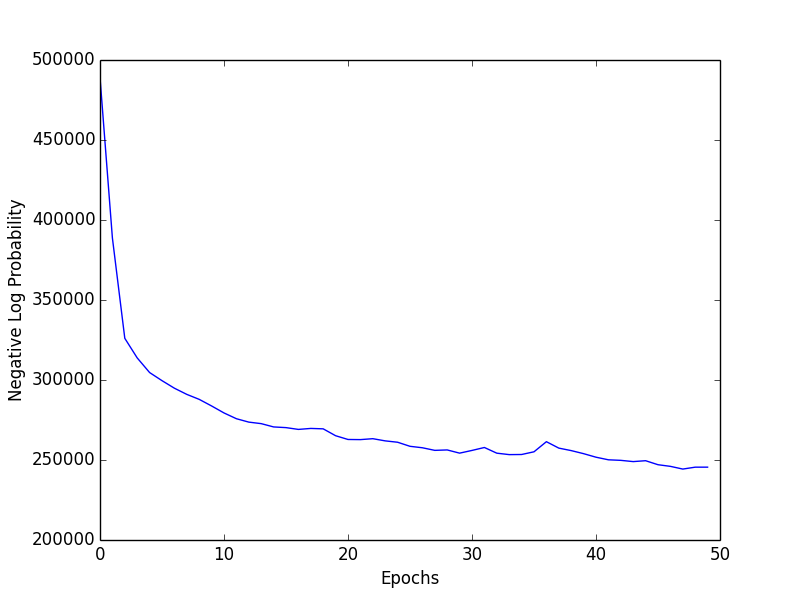
\includegraphics[width=0.45\textwidth]{logprob.png}
    \caption{Negative data log-likelihood}
\end{figure}
The fixed learning rate could be problematic, in that we observed \textit{unsmoothed} segments in the figure, which indicates that \textit{adadelta} or \textit{adaboost} should be taken into consideration.

Using the new trained phrase table and the default decoder, we obtained the worse score than given phrase table. The most reasonable explanation is that we are training on a too small data set with limited vocabulary($1500$) size, also the rescoring could also need more thoughts, since the simple softmax log-probability add gives quite similar scores, and is dominated by the length of the words.
%TODO
% subsection experiment (end)

\subsection{Conclusion} % (fold)
\label{sub:evaluation} 
Due to the substantial time needed for the training process, we are only able to conduct the experiment on a limited number of phrase pairs. Nevertehless the empirial experiments indicate that this model has large potential for the decoding task. 

Currently we are thinking of trying this model on a Germen-English phrase table extracted from the Moses, which gives us larger vocabulary and more training materials. Hopefully we could find some better training resources in the future. Besides, incorpating a better neural language model into the current architecture should also potentially yield a better performance.
% subsection evaluation (end)

\begin{thebibliography}{} \itemsep 0.3em

\bibitem[\protect\citename{Philipp Koehn.}2009]{phi}
Philipp Koehn.
\newblock {\em Statistical machine translation}.
\newblock 2009.
\newblock {Cambridge University Press.}

\bibitem[\protect\citename{Cho, K. et al.}2014]{rnn}
Cho, K., van Merrienboer, B., Gulcehre, C., Bougares, F., Schwenk, H., \& Bengio, Y.
\newblock (2014).
\newblock {Learning phrase representations using rnn encoder-decoder for statistical machine translation.}
\newblock {\textit{arXiv preprint arXiv:1406.1078.}}

\bibitem[\protect\citename{Mikolov, T.}2012]{bp}
Mikolov, T.
\newblock (2012).
\newblock {Statistical language models based on neural networks.}
\newblock \textit{Presentation at Google, Mountain View, 2nd April.}

\bibitem[\protect\citename{Bastien et al.}2012]{theano}
Bastien, Fr{\'{e}}d{\'{e}}ric and Lamblin, Pascal and Pascanu, Razvan and Bergstra, James and Goodfellow, Ian J. and Bergeron, Arnaud and Bouchard, Nicolas and Bengio, Yoshua
\newblock (2012).
\newblock {Theano: new features and speed improvements}
\newblock \textit{Deep Learning and Unsupervised Feature Learning NIPS 2012 Workshop.}

\end{thebibliography}
\end{document}